\documentclass[tikz]{standalone}
\standaloneconfig{border=-0.8cm -1.35cm -0.8cm -0.45cm} 
\usepackage{pgfplots}

\begin{document}
  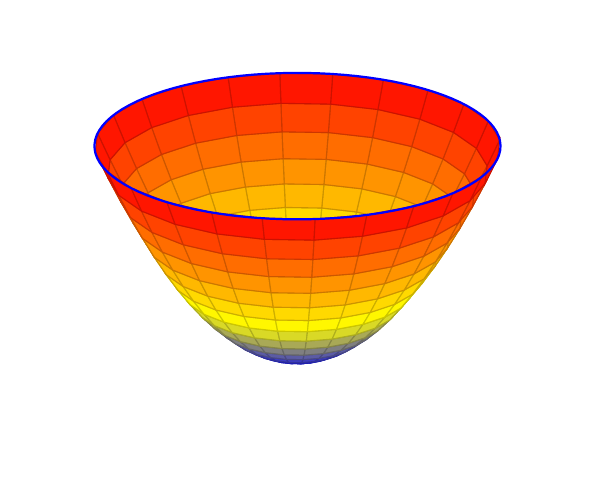
\begin{tikzpicture}
      \begin{axis} [
        xtick = {-50,-60},
        ytick = {-5,-6},
        ztick = {-3,-4},
        ticklabel style = {font = \scriptsize},
        axis line style={draw=none},
        tick style={draw=none}
      ]
      \addplot3 [surf,draw=none,restrict z to domain=0:4, data cs=polar, domain=0:360, y domain=0:3] (x, y, y^2);
      \addplot3[blue, thick, samples = 100, variable=t,domain=0:2*pi] (2*cos(deg(t)),{2*sin(deg(t))}, 4);
      \end{axis}
    \end{tikzpicture}
\end{document}
